\section{Shortcut-Modulated Looped Models for Latent Reasoning}
\label{sec:method}


\subsection{Notation and Problem Statement}

We denote by $X = (x_1, \dots, x_T)$ a sequence of $T$ tokens drawn from a vocabulary $\mathcal{V}$. The token embeddings are obtained via $E_{\text{tok}}(X) \in \mathbb{R}^{T \times d}$. Without loss of generality, positional embeddings can be added in a one-shot manner or applied through alternatives such as RoPE; in this work, we adopt the former for simplicity. The initial hidden states are therefore
\[
h^{(0)} \;=\; E_{\text{tok}}(X)\;+\;E_{\text{pos}}[1{:}T] \;\in\; \mathbb{R}^{T\times d}.
\]

A range of looping mechanisms for looped Transformers has been studied in prior work \cite{takase2021lessons, saunshi2025reasoning, bae2025mixture, bae2024relaxed}, including cycle, middle-cycle, and relaxed-cycle variants. Since our focus is on trajectories and their representation dynamics, we adopt the simplest \emph{cycle} design, where a stack of $k$ Transformer blocks, denoted by $\Phi_k(\cdot)$, is recursively applied on the hidden state. Following \cite{saunshi2025reasoning}, we write $(k \otimes L)$ for a looped model with $k$ blocks repeated $L$ times (approximate cost $kL$ FLOPs), and $(kL \otimes 1)$ for a non-looped Transformer of comparable depth.

LoopFormer applies $\Phi_k(\cdot)$ for $M$ iterations ($1 \le M \le L$), conditioning each loop $i$ on the pair $(t_{i-1}, \Delta_i)$, where $0 = t_0 < t_1 < \cdots < t_M = 1$ are cumulative normalized timesteps, and $\Delta_i = t_i - t_{i-1}$ is the step size of the $i$-th iteration. We refer to $\boldsymbol{\Delta_M} = (\Delta_1, \dots, \Delta_M)$ as a \emph{trajectory}, constrained by $\sum_{i=1}^M \Delta_i = 1$.

The \emph{maximum trajectory} corresponds to $L$ uniform steps with $\Delta_i = \frac{1}{L}$ for all $i$. At inference, a user specifies a compute budget $M$ and provides a step schedule $\boldsymbol{\Delta_M}$ such that $\sum_{i=1}^M \Delta_i = 1$.



% \begin{figure}[htbp]
%   \centering

%   \begin{subfigure}[t]{0.48\textwidth}
%     \centering
%     
\includegraphics[width=\linewidth]{assets/architecture.pdf}
%     \subcaption{Model architecture}
%     \label{fig:architecture}
%   \end{subfigure}
%   \hfill
%   \begin{subfigure}[t]{0.48\textwidth}
%     \centering
%     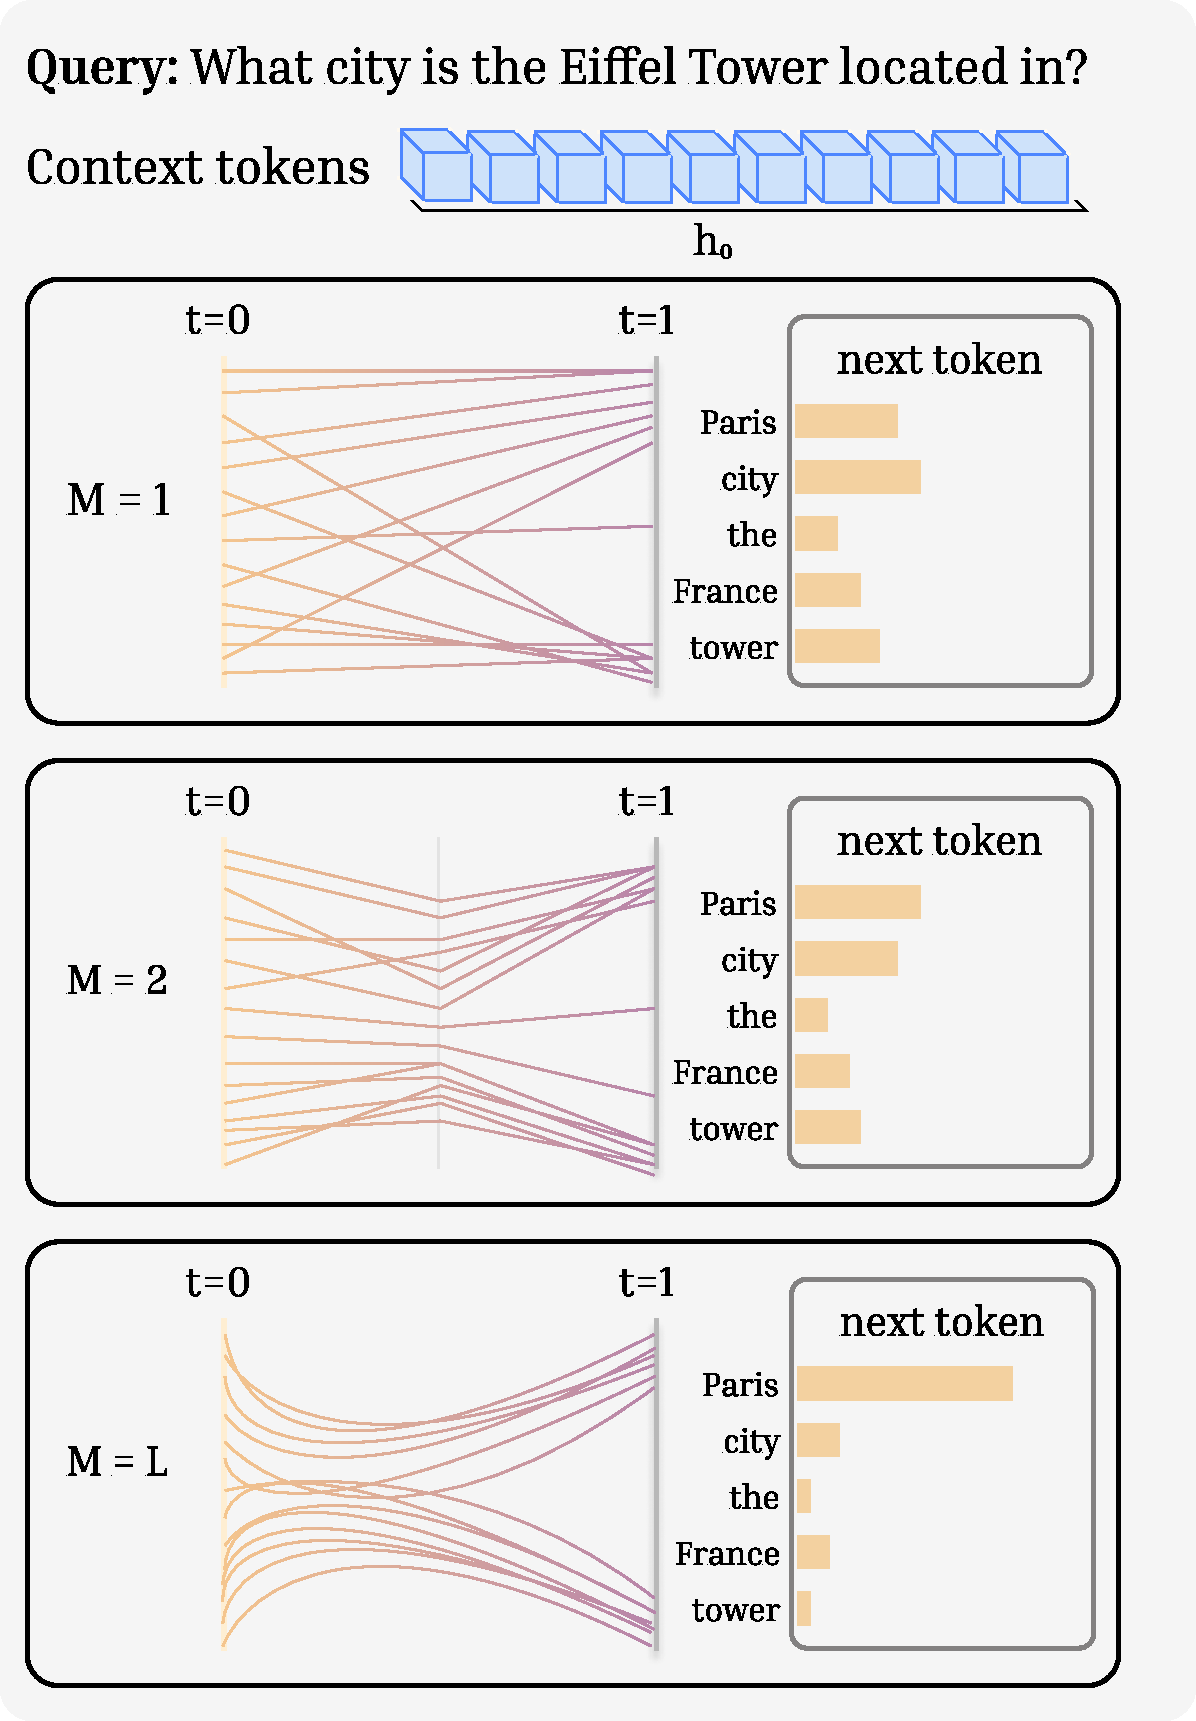
\includegraphics[width=\linewidth]{assets/trajectories.pdf}
%     \subcaption{Trajectory visualization}
%     \label{fig:trajectories}
%   \end{subfigure}

%   \caption{Overview of the system: (a) high-level model architecture; (b) example trajectories showing how different paths refine token distributions over steps.}
%   \label{fig:arch_and_traj}
% \end{figure}

\begin{figure}[t]
  \centering

  \begin{subfigure}[t]{0.48\textwidth}
    \centering
    
\includegraphics[width=\linewidth]{assets/architecture.pdf}
    \subcaption{LoopFormer architecture}
    \label{fig:architecture}
  \end{subfigure}
  \hfill
  \begin{subfigure}[t]{0.48\textwidth}
    \centering
    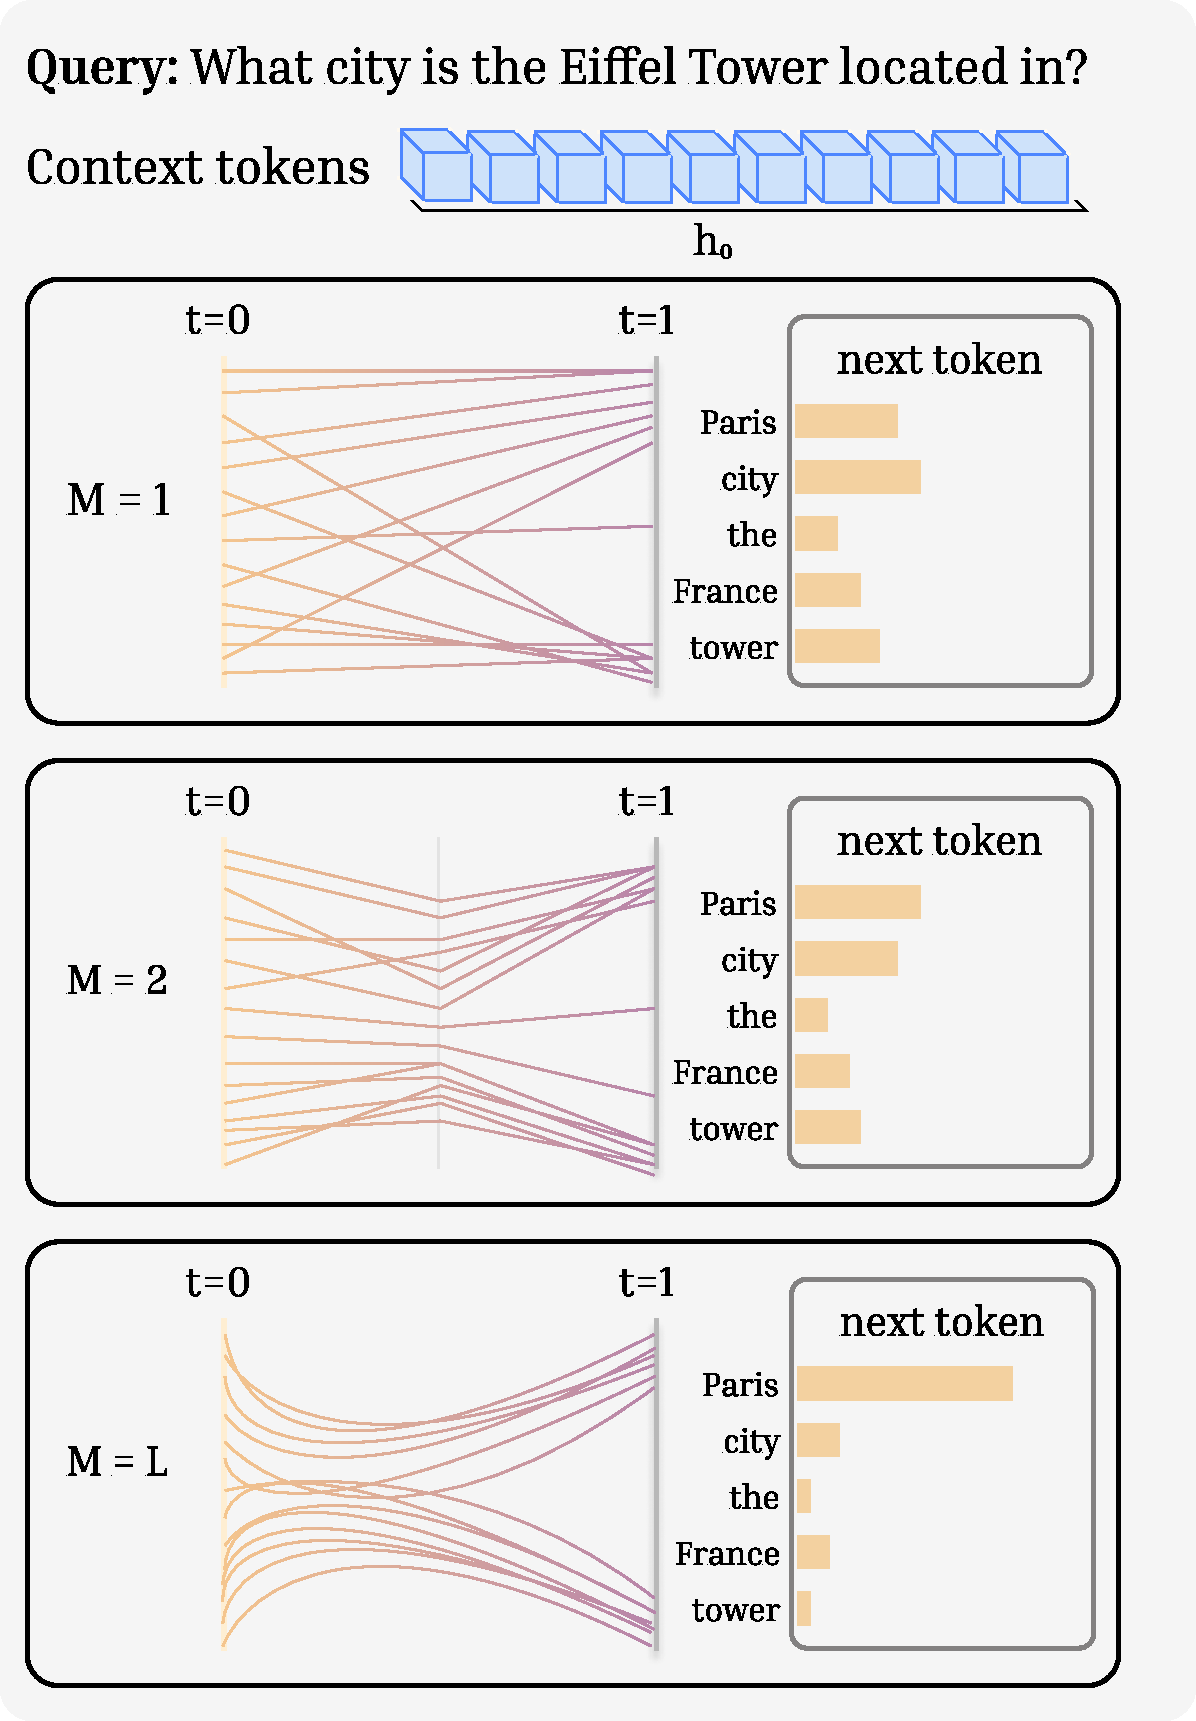
\includegraphics[width=\linewidth]{assets/trajectories.pdf}
    \subcaption{Budget-conditioned trajectories}
    \label{fig:trajectories}
  \end{subfigure}

  \caption{\textbf{(a)} LoopFormer conditions each loop on normalized time $t$ and step size $\Delta t$, modulating RMSNorm scales and gating the MHSA/FFN residuals. \textbf{(b)} During inference, shorter-budget trajectories ($M<L$) approximate the full $L$-step route; more budget yields progressively refined next-token distributions while preserving utility at low budget.}
  \label{fig:arch_and_traj}
\end{figure}


\subsection{Architecture}

We introduce \textbf{LoopFormer}, a looped language modeling architecture designed to remain faithful to the standard Transformer while incorporating trajectory-based conditioning. \autoref{fig:architecture} provides an overview. In this section we describe the forward pass and the core components of the model.

LoopFormer is a looped decoder-only Transformer in which a single shared stack is applied iteratively; the key novelty is \emph{how each loop is conditioned}. At iteration $i$, the model conditions on the pair $(t_{i-1},\Delta_i)$, where $t_{i-1}\in[0,1]$ is the cumulative normalized time and $\Delta_i\in(0,1]$ is the step size. Both scalars are encoded with sine–cosine frequency embeddings and projected by small MLPs to obtain $e_t$ and $e_\Delta$, which are summed to form $e_i=e_t+e_\Delta$. This signal modulates the \emph{LoopFormer Block}: an MLP maps $e_i$ to scaling $(\gamma_1,\gamma_2)$ for the two RMSNorm layers and to gating $(\alpha_1,\alpha_2)$ applied immediately before the residual connections of MHSA and FFN. As a result, each loop is explicitly aware of its location and granularity in the trajectory, enabling consistent behavior across coarse- and fine-grained schedules.

\paragraph{Relation to prior work.}
For the design of our architecture, we follow the overall approach of looped models such as ALBERT and recent looped decoders \cite{lan2019albert, saunshi2025reasoning}, and focus our novelty on \emph{trajectory conditioning}. Our modulation mechanism is inspired by Diffusion Transformers (DiT) \cite{peebles2023scalable} and shortcut/one-step diffusion \cite{frans2024one}, which condition blocks on a timestep via adaptive normalization (adaLN), regressing scale/shift and gates from a time embedding. In the looped language model setting, TMLT \cite{xu2024expressive} adopts this DiT-style idea by using the loop index as time (with RMSNorm). LoopFormer extends this conditioning by using both normalized time $t$ and step size $\Delta t$, and by training over families of trajectories with a shortcut-consistency objective, yielding trajectory-consistent representations suitable for budget-conditioned inference.


% LoopFormer follows the overall structure of existing looped models such as ALBERT \cite{lan2019albert} and \cite{saunshi2025reasoning}, and we adopt the open-source GPT-2 implementation by NanoGPT as a reference backbone. The main novelty lies in how each loop is conditioned, through what we call the \emph{LoopFormer Block}. Its design is inspired by Diffusion Transformers~\cite{peebles2023scalable}, which condition blocks on timesteps $t$ and replace standard layer normalization with adaptive layer normalization (adaLN), where the scaling, shifting, and gating parameters $(\gamma, \beta, \alpha)$ are produced via lightweight regressors. Recent work on Time-Modulated Looped Transformers (TMLT)~\cite{xu2024expressive} applied this idea to looped models, using RMSNorm in place of LayerNorm and conditioning on the loop index as a proxy for time.

% We build upon this line of work, but extend it beyond fixed loop indices. Conditioning only on loop number, as in TMLT, still restricts models to a static trajectory. By contrast, LoopFormer conditions each loop $i$ on the pair $(t_{i-1}, \Delta_i)$ defined in the previous subsection, where $t_{i-1} \in [0,1]$ is the normalized cumulative time and $\Delta_i \in (0,1]$ is the step size. Both scalars are first encoded via sine–cosine frequency embeddings, then projected through MLPs to produce embeddings $e_t$ and $e_\Delta$. Their sum $e_i = e_t + e_\Delta$ serves as the conditioning signal for the $i$-th loop. 

% Following the design of DiT and TMLT blocks, $e_i$ is further transformed by an MLP to generate modulation parameters: scaling coefficients $(\gamma_1, \gamma_2)$ for the two RMSNorm layers and gating coefficients $(\alpha_1, \alpha_2)$ applied directly before residual connections. This conditioning mechanism ensures that each loop step is explicitly aware of both its location in the trajectory and its step size, enabling LoopFormer to represent coarse- and fine-grained trajectories consistently.



\subsection{Training \& Inference with LoopFormer}

A key goal of LoopFormer is to train models that perform well even with fewer than $L$ loops, thereby enabling \emph{elastic depth} at inference time. Unlike prior adaptive-compute approaches that rely on per-token halting or early exits, our framework uses a user-defined compute budget, similar in spirit to diffusion models. Empirically, we find that naive early exiting in looped architectures leads to \emph{stagnant} representations in later iterations, under-utilizing depth. To address this, LoopFormer leverages shortcut conditioning together with a consistency loss that encourages trajectories of different lengths to converge toward the full trajectory of length $L$. The overall objective is:
\[
  \mathcal{L}
  \;=\;
  \mathcal{L}_{\text{L}}
  \;+\;
  \lambda_1\,\mathcal{L}_{\text{S}}
  \;+\;
  \lambda_2\,\mathcal{L}_{\text{cons}},
\]
where $\mathcal{L}_{\text{L}}$ and $\mathcal{L}_{\text{S}}$ denote next-token prediction losses for the longest and sampled shortcut trajectories, respectively, and $\mathcal{L}_{\text{cons}}$ is a stop-gradient consistency loss aligning per-token logits of shorter trajectories to those of the longest trajectory. We set $\lambda_{1}=\lambda_{2}=0.1$ in all experiments. Algorithm~\ref{alg:training} formalizes the training procedure.

\paragraph{Shortcut trajectory sampling.}
Given a LoopFormer $(k \otimes L)$ and the maximum trajectory $\boldsymbol{\Delta_L}$, during training, we additionally sample a shortcut trajectory $\boldsymbol{\Delta_S}$ with budget $1 \le S < L$. For simplicity, at each batch we first sample a shortcut length $S \sim \mathcal{U}\{1, \ldots, L-1\}$, then uniformly draw the discrete step schedule $\boldsymbol{\Delta_S}$ over $[0,1]$ such that $\sum_{i=1}^S \Delta_i = 1$. This ensures exposure to both long and short trajectories during training.

\paragraph{Inference with elastic depth.}
At inference time, LoopFormer can be deployed flexibly at any budget $M \le L$. A user specifies $M$ and  $\boldsymbol{\Delta_M}$, and the model produces outputs that scale smoothly with compute, without retraining. \autoref{fig:trajectories} provides a conceptual illustration of budget-conditioned refinement: for any chosen budget, shorter routes are trained to approximate the $t{=}1$ endpoint, with quality improving as steps increase. Algorithm~\ref{alg:inference} outlines the inference procedure.




% In Section~\ref{sec:experiments} we analyze the impact of varying $M$ and trajectory on representation dynamics and provide oracle studies on the average number of loops required for different tasks.




\begin{figure}[t]
\centering
\begin{minipage}[t]{0.56\textwidth}
\begin{algorithm}[H]
\caption{LoopFormer Training}
\label{alg:training}
\begin{algorithmic}
\While{not converged}
  \State Sample batch $(X, Y)$
  \State Construct max trajectory $\boldsymbol{\Delta_L}$
  \State Sample shortcut length $S \sim \mathcal{U}\{1, \ldots, L-1\}$
  
  \State Sample trajectory $\boldsymbol{\Delta_S}$ of length $S$

  \State $h^{(L)} \gets \Phi_k(h^{(0)};\boldsymbol{\Delta_L})$ \;; $h^{(S)} \gets \Phi_k(h^{(0)};\boldsymbol{\Delta_S})$
  
  \State $\mathcal{L}_L \gets \mathrm{CE}(\mathrm{LMHead}(h^{(L)}), Y)$
  
  \State $\mathcal{L}_S \gets \mathrm{CE}(\mathrm{LMHead}(h^{(S)}), Y)$
  \State $\mathcal{L}_{\mathrm{cons}} \gets 
         \| \operatorname{stopgrad}(h^{(L)}) - h^{(S)} \|^2$
  \State Update $\theta$ using $\nabla_\theta\big(\mathcal{L}_L + \lambda_1 \mathcal{L}_S + \lambda_2 \mathcal{L}_{\mathrm{cons}}\big)$
\EndWhile
\end{algorithmic}
\end{algorithm}
\end{minipage}
\hfill
\begin{minipage}[t]{0.40\textwidth}
\begin{algorithm}[H]
\caption{LoopFormer Inference}
\label{alg:inference}
\begin{algorithmic}
\State Given input $X$ 
\State Choose budget $M \le L$
\State Sample schedule $\boldsymbol{\Delta_M}$
\State Initialize $h^{(0)} \gets E_{\mathrm{tok}}(X) + E_{\mathrm{pos}}$
\For{$i=1$ to $M$}
  \State $h^{(i)} \gets \Phi_k\!\big(h^{(i-1)}; t_{i-1}, \Delta_i\big)$
\EndFor
\State \Return $\mathrm{LMHead}(h^{(M)}[:,-1])$
\end{algorithmic}
\end{algorithm}
\end{minipage}
\end{figure}






